\subsection{Beleuchtung}
\label{subsec:Beleuchtung_2}

Damit die Maschine schon von Weitem erkennbar ist, wird ein auffallendes Mittel benötigt. Dazu eignet sich ein LED-Band hervorragend, am besten wenn es noch verschiedenfarbig ist. Dazu ist einerseits das LED-Band von Nöten und die geeignete Ansterung dazu. Für die Cocktailmaschine wurde festgelegt, dass der LED-Streifen die benötigten Wirderstände für die LED's schon aufgeklebt hat und die Ansteuerung folglich direkt über FET's geschehen kann. Der Aufbau ähnelt dann dem in Abbildung \ref{fig:LED1} gezeigten Schaltung. Der Streifen wäre Rot eingerahmt, die LED's und Widerstände befinden sich auf dem Band und die zu sehenden Fähnchen für R, G, B und W führen zum Mikrocontroller. Es können auch mehrere Bänder parallel geschaltet werden, wie in Abbildung \ref{fig:LED1} ersichtlich ist.

\begin{figure}[h!]
\center
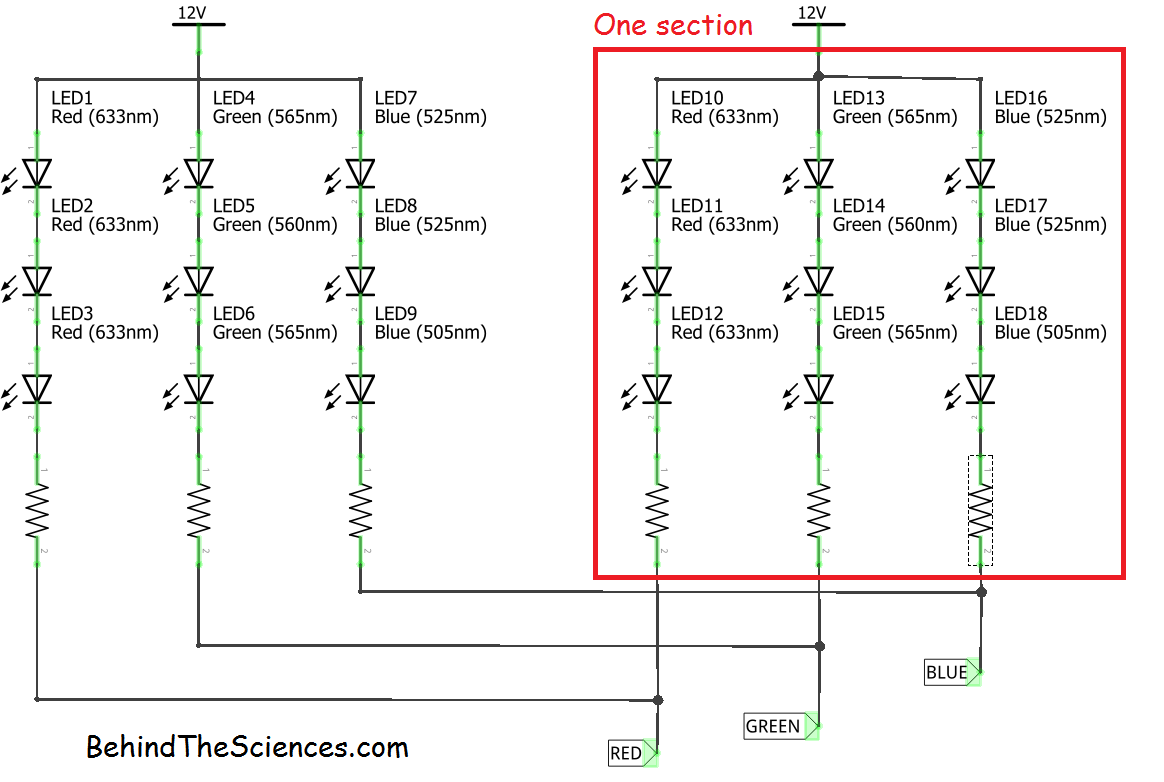
\includegraphics[width = 0.5\textwidth]{graphics/Schema_LED1}
\caption{LED Beispiel.}
\label{fig:LED1}
\end{figure}

\paragraph{Schema}\mbox{}

Abbildung \ref{fig:Schema_LED} zeigt den Schaltungsaufbar der LED-Steuerung. Damit die LED's angesteuert werden können, braucht es ein Bauteil, welches mit einer 5V-Ansteuerung 12V schalten können. Dazu wird ein MOSFET verwendet. Über die Widerstände an den Gates wird der Strom zum Schutz des Gates begrenzt. Die Leitungen führen direkt auf den Klemmblock für die LED-Streifen. Parallel dazu wurden noch für jede Lichtfarbe ein Kontroll-LED installiert, welche es ermöglicht auch ohne LED-Band etwas zu programmieren.

\begin{figure}[!h]
\center
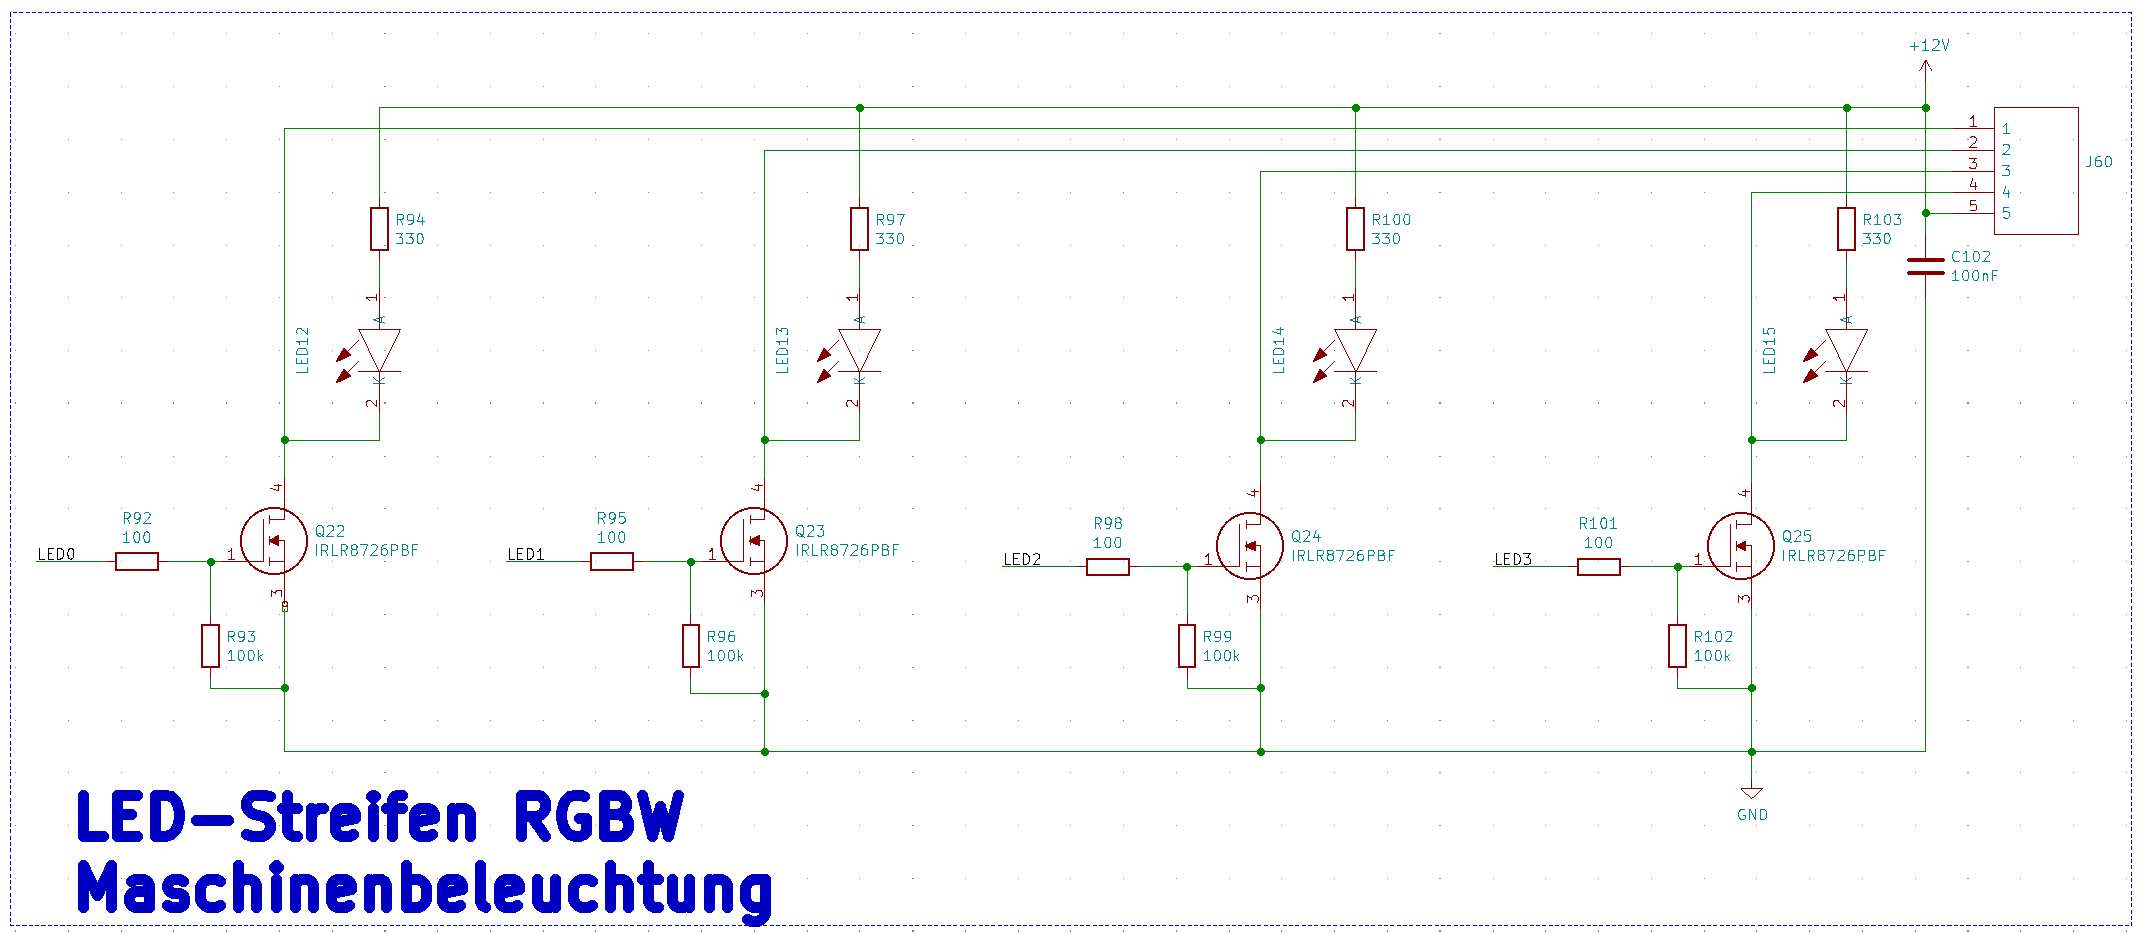
\includegraphics[width =  \textwidth]{graphics/Schema_LED}
\caption{Schema der LED-Ansteuerung}
\label{fig:Schema_LED}
\end{figure}
\newpage
\paragraph{Funktionsbeschrieb der Schaltung}\mbox{}

Licht sind bekanntlich elektromagnetische Wellen im sichtbaren Wellenlängen-Bereich. Dabei gibt es vier Hauptfarben: Rot, Grün, Blau und Weiss. Zwar kann Weiss auch aus einer Kombination aller drei Farben erstellt werden, kommt aber besser mit einer separaten Diode. Das resultierende Licht des Bandes ist eine Überlagerung der Wellenlängen. Diese Überlagerung kann vom Mikrocontroller über den Duty-Cycle eines PWM-Signals gesteuert werden. So lassen sich mit dem Licht praktisch aus den Grundfarben praktisch alle Farben mischen.